%-----------------------------QUESTÃO------------------------------------
%Cód.: TF3p05q24

\question  Determine o módulo da força de interação entre duas
partículas eletrizadas com $q_1=\SI{+4,0e-6}{\coulomb}$ e $q_2=\SI{3,0e-6}{\coulomb}$, estando elas no vácuo à
distância de \SI{6,0e-2}{\meter} {\small (6 centímetros)} uma da outra.\\
Dados:\\
Constante eletrostática do vácuo $k=\SI{9e9}{\newton\meter^2\per\coulomb^2}$\\
Força Elétrica: $F_e=k\times\frac{ q_1 \times q_2 }{ d^{2}} 
				$

%------------------------------ALTERNATIVAS-----------------------------

		\begin{EnvUplevel}
			\begin{choices}
			
			\choice \SI{10}{\newton}  
			\choice \SI{20}{\newton}
			\correctchoice \SI{30}{\newton}
			\choice \SI{40}{\newton}
			\choice \SI{50}{\newton}
				
			\end{choices}
		\end{EnvUplevel}

%--------------------------SOLUÇÃO---------------------------------------
		
		\begin{EnvUplevel}
		\begin{solution}[2cm]
		{\footnotesize
		Como as cargas têm sinais opostos, a interação entre elas é atrativa.
		
		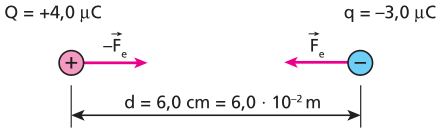
\includegraphics[width=0.4\linewidth]{questoes/imagens/TF3p05q24_1}
	
		Aplicando a Lei de Coulomb a essa interação, temos:
				$$
				F_e=k\times\frac{\left| Q \times q \right|}{\left( d \right)^{2}} \\
				$$
		Substituindo os valores conhecidos, vem:
				$$
				F_e=\num{9e9}\times\frac{\left| \num{4,0e-6} \times \num{3,0e-6} \right|}{\left( \num{6,0e-2} \right)^{2}}
				$$
				$$
				F_e=\SI{30}{\newton}
				$$
		}
		
		\end{solution}
		\end{EnvUplevel}
